% =====================================================================
% Quorum — Software Project Report
% CSE 3422 Software Engineering Laboratory — Section C
% =====================================================================
\documentclass[11pt,a4paper]{article}

\usepackage[utf8]{inputenc}
\usepackage[T1]{fontenc}
\usepackage[margin=2.5cm]{geometry}
\usepackage{graphicx}
\usepackage{booktabs}
\usepackage{longtable}
\usepackage{array}
\usepackage{tabularx}
\usepackage{enumitem}
\usepackage{caption}
\usepackage{xcolor}
\usepackage{tikz}
\usepackage{titlesec}
\usepackage[hidelinks]{hyperref}
\usetikzlibrary{arrows.meta,positioning,shapes.geometric,backgrounds,fit}

\definecolor{quorumviolet}{RGB}{113,96,220}
\definecolor{quorumgreen}{RGB}{62,207,110}
\definecolor{quorumdark}{RGB}{18,21,28}

% ---------------------------------------------------------------------
% Title page
% ---------------------------------------------------------------------
\title{\vspace{-1.2cm}\textbf{Quorum}\\[0.3cm]
  \large AI-Powered GitHub Pull Request Review and Analysis System\\[0.2cm]
  \normalsize Software Project Report\\[0.6cm]}
\author{
  Saiful Alam (0112320105)\\
  Sabbir Ahmed (011222279)\\[0.5cm]
  \normalsize CSE 3422 --- Software Engineering Laboratory, Section C\\
  \normalsize Faculty: Zobaer Ibn Razzaque
}
\date{\today}

% ---------------------------------------------------------------------
% Helper: include a screenshot if present, otherwise a placeholder box
% ---------------------------------------------------------------------
\newcommand{\reportfigure}[4]{%
  \begin{figure}[htbp]
    \centering
    \IfFileExists{screenshots/#1}{%
      \includegraphics[width=\textwidth]{screenshots/#1}%
    }{%
      \fcolorbox{black!25}{black!6}{%
        \parbox[c][6cm][c]{0.92\textwidth}{%
          \centering\itshape Screenshot placeholder ---\\ #2}}%
    }
    \caption{#2 --- #4}\label{#3}
  \end{figure}
}

\setlength{\parindent}{0pt}
\setlength{\parskip}{6pt}

\begin{document}

\maketitle
\thispagestyle{empty}
\newpage

\tableofcontents
\newpage

\section{Project Introduction / Objective}
\subsection{What Quorum Is}

Quorum is an AI-powered GitHub Pull Request review system. It is a web
application that automatically analyzes pull requests opened in a GitHub
repository, produces a deterministic Merge Readiness Score, and presents the
results in a web dashboard with an evidence-grounded question-answering
assistant called \emph{Ask Quorum}. The system is implemented as a Python /
FastAPI backend, a React/TypeScript frontend, and a PostgreSQL database, and
it integrates with GitHub through a GitHub App, OAuth authentication, and
webhooks.

\subsection{The Problem Addressed}

Reviewing a pull request manually is time-consuming and error-prone. A
reviewer must inspect the changed code, look for security problems, estimate
whether the change might break existing behaviour, and form an opinion about
whether the change is safe to merge. This judgement is often based on
subjective impressions rather than measured evidence, and it is easy to miss
a security issue or a failing test. The conventional review process also
requires the reviewer to either write and run tests manually or trust the
author's claims.

\subsection{What Quorum Automates}

Quorum automates the evidence-gathering part of code review. When a pull
request event reaches the backend, the orchestrator runs a review pipeline
that:

\begin{itemize}
  \item extracts and parses the pull request diff and the changed Python
        files (diff and AST analysis);
  \item runs the \textbf{Semgrep} static analysis tool over the changed files
        to obtain security evidence;
  \item passes the Semgrep findings and code context to a \textbf{Security
        Agent} (an LLM-driven agent) which reasons over the evidence and
        produces structured, evidence-traceable security findings;
  \item uses a \textbf{Test Writer Agent} to generate \texttt{pytest} tests
        for the modified functions;
  \item executes the generated tests inside an isolated, hardened
        \textbf{Docker sandbox} and measures code coverage before and after;
  \item combines the security, test, and coverage results into a
        deterministic \textbf{Merge Readiness Score} from 0 to 100;
  \item persists the results in PostgreSQL and posts a concise review summary
        back to the pull request on GitHub.
\end{itemize}

\subsection{How the Result Helps Developers}

The Merge Readiness Score is deterministic: the same evidence always produces
the same score, and the breakdown (security findings, generated tests, and
coverage) is stored with the analysis. A developer can therefore look at a
pull request and immediately understand both the score and the reasons behind
it, rather than relying on an unverifiable subjective opinion. The dashboard
shows security findings with evidence, generated test outcomes, coverage
deltas, and the score for each pull request, and the Ask Quorum assistant
answers questions about a specific review using only that review's stored
evidence.

\subsection{The Role of the Dashboard}

The React dashboard is the visual control centre for the pipeline. It allows a
signed-in user to discover and connect GitHub repositories, open a repository
workspace, create and manage pull requests (including creating, merging, and
closing them from Quorum), view per-pull-request analysis results, review
history, security findings, and settings, and ask questions about a review.

\subsection{Project Objective}

The overall objective of the project is to provide an end-to-end,
evidence-based pull request review tool that helps developers assess whether a
change is safe to merge. The project demonstrates the combination of static
security analysis, LLM-driven reasoning, automated test generation, sandboxed
test execution, coverage measurement, and deterministic result synthesis, all
presented through a multi-user web application integrated with GitHub.

\subsection{Implementation Status}

All planned roadmap phases (Phase 0 through Phase 19) are implemented. The
LLM layer is active through the OpenAI provider; a local \texttt{Ollama}
provider exists in the codebase but is not currently used. Components that are
planned but not yet implemented (such as an automated CI pipeline and a backup
demo video) are noted in the project documentation as future work.

\section{Functional Requirements}
The functional requirements below describe the behaviour that is currently
implemented in the Quorum codebase. Each requirement is identified by a code
(\texttt{FR-NN}) and its implementation status is stated explicitly. Nothing
is listed here that is not actually implemented.

\subsection{A. Authentication and Authorization}

\begin{longtable}{@{}p{1.4cm}p{11.6cm}p{2.0cm}@{}}
\toprule
\textbf{ID} & \textbf{Requirement} & \textbf{Status} \\
\midrule
\endhead
FR-01 & The system shall allow a user to sign in using GitHub OAuth through the
\emph{Continue with GitHub} flow. & Implemented \\
FR-02 & The system shall create a server-side session after a successful OAuth
callback and clear it on logout. & Implemented \\
FR-03 & The system shall expose the current user's profile through
\texttt{GET /api/me}. & Implemented \\
FR-04 & The system shall accept the GitHub App installation callback
(\texttt{GET /auth/install-callback}) to record the installation and return
the user to Quorum with a connection result. & Implemented \\
\bottomrule
\end{longtable}

\subsection{B. GitHub Integration}

\begin{longtable}{@{}p{1.4cm}p{11.6cm}p{2.0cm}@{}}
\toprule
\textbf{ID} & \textbf{Requirement} & \textbf{Status} \\
\midrule
\endhead
FR-05 & The system shall verify every GitHub webhook request using the HMAC
SHA-256 signature (\texttt{X-Hub-Signature-256}). & Implemented \\
FR-06 & The system shall handle \texttt{pull\_request} webhook events
(\texttt{opened}, \texttt{reopened}, \texttt{synchronize}, \texttt{closed}),
persist the pull request, and schedule analysis in the background. & Implemented \\
FR-07 & The system shall use the GitHub App installation token for
installation-scoped GitHub API calls. & Implemented \\
FR-08 & The system shall post a concise review summary comment back to the pull
request on GitHub after analysis. & Implemented \\
FR-09 & The system shall create real pull requests on GitHub from the Quorum
dashboard (\texttt{POST /api/repositories/\{id\}/pull-requests}). & Implemented \\
FR-10 & The system shall merge and close pull requests on GitHub from the
Quorum dashboard, with an optional merge message. & Implemented \\
\bottomrule
\end{longtable}

\subsection{C. Repository Management}

\begin{longtable}{@{}p{1.4cm}p{11.6cm}p{2.0cm}@{}}
\toprule
\textbf{ID} & \textbf{Requirement} & \textbf{Status} \\
\midrule
\endhead
FR-11 & The system shall list the user's GitHub repositories with their
connected status (\texttt{GET /api/repositories/discover}). & Implemented \\
FR-12 & The system shall connect and disconnect repositories through the
GitHub App installation flow, using a popup and confirmation banners. & Implemented \\
FR-13 & The system shall remember intentional disconnects so that automatic
re-syncs do not re-attach a repository. & Implemented \\
FR-14 & The system shall provide a per-repository workspace page that lists the
repository's pull requests and offers a create-pull-request entry point. & Implemented \\
\bottomrule
\end{longtable}

\subsection{D. Pull Request Processing}

\begin{longtable}{@{}p{1.4cm}p{11.6cm}p{2.0cm}@{}}
\toprule
\textbf{ID} & \textbf{Requirement} & \textbf{Status} \\
\midrule
\endhead
FR-15 & The system shall list the branches of a connected repository
(\texttt{GET /api/repositories/\{id\}/branches}). & Implemented \\
FR-16 & The create-pull-request form shall let the user choose a Base and a
Compare branch and shall auto-suggest a title from the compare branch. & Implemented \\
FR-17 & The system shall reconcile a pull request's state from GitHub when the
stored copy is stale, so that pull requests closed or merged on GitHub appear
correctly in Quorum. & Implemented \\
\bottomrule
\end{longtable}

\subsection{E. Automated Analysis Pipeline}

\begin{longtable}{@{}p{1.4cm}p{11.6cm}p{2.0cm}@{}}
\toprule
\textbf{ID} & \textbf{Requirement} & \textbf{Status} \\
\midrule
\endhead
FR-18 & The system shall run the review pipeline through an orchestrator with
registered stages and a persistent analysis-run lifecycle. & Implemented \\
FR-19 & The system shall fetch and parse the unified diff of a pull request. & Implemented \\
FR-20 & The system shall parse changed Python files with the standard \texttt{ast}
module to identify modified functions and classes. & Implemented \\
FR-21 & The system shall build a bounded, prioritized context from the changed
files (context-window management). & Implemented \\
\bottomrule
\end{longtable}

\subsection{F. Security Analysis}

\begin{longtable}{@{}p{1.4cm}p{11.6cm}p{2.0cm}@{}}
\toprule
\textbf{ID} & \textbf{Requirement} & \textbf{Status} \\
\midrule
\endhead
FR-22 & The system shall run \texttt{Semgrep} over the changed files and parse
its JSON findings into a structured evidence model. & Implemented \\
FR-23 & The system shall run a Security Agent that reasons over the Semgrep
evidence and the code context, and whose findings must be traceable to that
evidence. & Implemented \\
FR-24 & The system shall persist security findings with severity, file, line,
evidence, and explanation. & Implemented \\
\bottomrule
\end{longtable}

\subsection{G. Test Generation and Execution}

\begin{longtable}{@{}p{1.4cm}p{11.6cm}p{2.0cm}@{}}
\toprule
\textbf{ID} & \textbf{Requirement} & \textbf{Status} \\
\midrule
\endhead
FR-25 & The system shall generate \texttt{pytest} tests for modified Python
functions using a Test Writer agent, with syntax validation. & Implemented \\
FR-26 & The system shall execute generated tests inside a hardened Docker
sandbox (no network, memory/process limits, hard timeout, cleanup). & Implemented \\
FR-27 & The system shall measure code coverage before and after the generated
tests and compute the coverage delta. & Implemented \\
\bottomrule
\end{longtable}

\subsection{H. Analysis Results and Scoring}

\begin{longtable}{@{}p{1.4cm}p{11.6cm}p{2.0cm}@{}}
\toprule
\textbf{ID} & \textbf{Requirement} & \textbf{Status} \\
\midrule
\endhead
FR-28 & The system shall compute a deterministic Merge Readiness Score from 0
to 100 from the security, test, and coverage evidence, without LLM
involvement. & Implemented \\
FR-29 & The system shall persist the score and its breakdown (security, test,
and coverage deductions) with the analysis run. & Implemented \\
FR-30 & For pull requests with no changed Python files (for example
documentation-only changes), the system shall skip the test and coverage
deductions because they are not applicable. & Implemented \\
\bottomrule
\end{longtable}

\subsection{I. Dashboard}

\begin{longtable}{@{}p{1.4cm}p{11.6cm}p{2.0cm}@{}}
\toprule
\textbf{ID} & \textbf{Requirement} & \textbf{Status} \\
\midrule
\endhead
FR-31 & The dashboard shall show overview metrics, the user's repositories,
and pull requests that need attention. & Implemented \\
FR-32 & The dashboard shall list pull requests with their latest analysis
status and score, and link to a detailed review page. & Implemented \\
FR-33 & The dashboard shall display security findings across repositories and
the review history. & Implemented \\
FR-34 & The repositories page shall force a fresh sync with GitHub when opened,
and background pages shall auto-refresh so that new results appear without a
manual refresh. & Implemented \\
\bottomrule
\end{longtable}

\subsection{J. Ask Quorum}

\begin{longtable}{@{}p{1.4cm}p{11.6cm}p{2.0cm}@{}}
\toprule
\textbf{ID} & \textbf{Requirement} & \textbf{Status} \\
\midrule
\endhead
FR-35 & The system shall provide a chat endpoint scoped to a specific review
(\texttt{GET}/\texttt{POST /api/reviews/\{id\}/chat}). & Implemented \\
FR-36 & The assistant shall answer only from the selected review's stored
evidence (findings, tests, coverage, and score breakdown) and treat repository
content as untrusted input (prompt-injection defense). & Implemented \\
FR-37 & The system shall persist chat messages and provide a full
\emph{Ask Quorum} page as well as a floating chat. & Implemented \\
\bottomrule
\end{longtable}

\subsection{K. Review History}

\begin{longtable}{@{}p{1.4cm}p{11.6cm}p{2.0cm}@{}}
\toprule
\textbf{ID} & \textbf{Requirement} & \textbf{Status} \\
\midrule
\endhead
FR-38 & The system shall list all analysis runs (reviews) with their score,
status, findings, tests, and coverage, and provide a review detail page. & Implemented \\
\bottomrule
\end{longtable}

\subsection{L. Settings and Profile}

\begin{longtable}{@{}p{1.4cm}p{11.6cm}p{2.0cm}@{}}
\toprule
\textbf{ID} & \textbf{Requirement} & \textbf{Status} \\
\midrule
\endhead
FR-39 & The system shall show the user's GitHub account, connected
repositories, and GitHub App authorization status, and allow the user to sign
out. & Implemented \\
\bottomrule
\end{longtable}

\section{Scope of the Project}
\subsection{In Scope}

The current Quorum project delivers the following, all of which are implemented
in the repository:

\begin{itemize}
  \item GitHub OAuth authentication and session management for the web
        application.
  \item GitHub App installation/authorization for repository access, including
        the installation callback, repository discovery, and one-click
        connect/disconnect flows with confirmation banners.
  \item Repository workspaces and pull request management from the dashboard,
        including creating pull requests (Base and Compare branches with
        suggested titles), and merging and closing pull requests with an
        optional merge message.
  \item Automated pull request analysis: diff extraction, Python AST
        analysis, bounded context management, Semgrep static security
        scanning, an LLM-driven Security Agent, an LLM-driven Test Writer, and
        sandboxed test execution with coverage measurement.
  \item A deterministic Merge Readiness Score (0--100) with a persisted
        breakdown, and an automatic GitHub review comment.
  \item PostgreSQL persistence of users, repositories, pull requests, analysis
        runs, security findings, test runs, coverage results, and chat
        messages, managed through Alembic migrations.
  \item A FastAPI REST API used by the dashboard for all reads and writes,
        with user-level access isolation.
  \item A React/TypeScript dashboard with landing page, dashboard,
        repositories, repository workspace, pull requests, PR review details,
        findings, review history, profile, settings, and Ask Quorum.
  \item An evidence-grounded Ask Quorum assistant scoped to the selected
        review.
  \item An evaluation harness (\texttt{evaluation/}) with deterministic
        metrics over a labeled pull request dataset.
  \item A local development setup using a Cloudflare quick tunnel to receive
        GitHub webhooks during development.
\end{itemize}

\subsection{Out of Scope}

The following are explicitly outside the scope of the current project and are
not implemented:

\begin{itemize}
  \item Replacing GitHub itself, or providing a Git hosting platform.
  \item Replacing human code review; Quorum provides evidence and a score but
        does not make a final merge decision for the user.
  \item Unrestricted repository administration, such as managing collaborators
        or repository settings.
  \item Full IDE functionality or arbitrary in-app code editing of the
        repository.
  \item A general-purpose chatbot; Ask Quorum is intentionally restricted to
        the evidence of the selected review.
  \item Automated CI/CD pipeline configuration (a basic CI pipeline is planned
        future work, not yet implemented).
  \item Automated deployment to a production hosting platform.
  \item Support for languages other than Python for test generation and
        coverage (Semgrep scanning is language-agnostic, but the AST, test
        writer, and coverage stages target Python).
\end{itemize}

These items are not claimed as implemented anywhere in this report; they are
documented here so that the scope of the project is unambiguous.

\section{Technology Stack}
The table below lists the technologies actually used in the Quorum
implementation. Each technology was verified against the repository
(requirements files, configuration, and source code).

\begin{longtable}{@{}p{3.4cm}p{5.4cm}p{6.6cm}@{}}
\toprule
\textbf{Layer} & \textbf{Technology} & \textbf{Usage} \\
\midrule
\endhead
Backend language & Python 3.13 & Main backend, analysis, orchestration \\
Backend framework & FastAPI & REST API and GitHub webhook server \\
ASGI server & Uvicorn & Runs the FastAPI application \\
Data validation & Pydantic & Request/response and model validation \\
Database & PostgreSQL & Persistent application/review/chat data \\
ORM & SQLAlchemy 2.0 & Database access \\
Migrations & Alembic & Database schema migrations \\
GitHub integration & GitHub App, OAuth, Webhooks, REST API & PR events, auth, installation access \\
HTTP client & httpx & GitHub and LLM communication \\
JWT & PyJWT & GitHub App authentication \\
Static analysis & Semgrep (v1.177) & Security evidence over changed files \\
Code analysis & Python standard \texttt{ast} & Structural analysis of changed Python code \\
LLM interface & \texttt{LLMProvider} abstraction & Security, test, and chat reasoning \\
LLM provider (active) & OpenAI (GPT-5.6 Terra / Luna) & Security Agent, Test Writer, Ask Quorum \\
LLM provider (dormant) & Ollama (Qwen2.5-Coder) & Optional local fallback, not in use \\
Test execution & Docker sandbox & Isolated execution of generated tests \\
Sandbox image & \texttt{quorum-sandbox} & pytest + pytest-cov image \\
Backend tests & pytest, pytest-cov & Automated backend tests \\
Frontend & React, TypeScript & Web dashboard \\
Frontend build & Vite & Fast development/build \\
Styling & Tailwind CSS & UI styling \\
UI components & shadcn-style design tokens & Reusable accessible UI components \\
Frontend tests & Vitest, React Testing Library & Component tests \\
Development webhook tunnel & Cloudflare Quick Tunnel & Expose local FastAPI to GitHub \\
\bottomrule
\end{longtable}

\subsection{LLM Configuration}

The LLM is accessed through a common \texttt{LLMProvider} interface so that
no agent depends on a concrete provider. The active provider is OpenAI, with
per-role models:

\begin{itemize}
  \item Security Agent $\rightarrow$ \texttt{gpt-5.6-terra}
  \item Test Writer $\rightarrow$ \texttt{gpt-5.6-terra}
  \item Ask Quorum $\rightarrow$ \texttt{gpt-5.6-luna}
\end{itemize}

A single \texttt{OPENAI\_API\_KEY} authenticates all roles and is stored only
server-side. The \texttt{OllamaProvider} exists in the codebase as an optional
local fallback but is not currently used.

\section{Software Architecture}
\subsection{Overview}

Quorum follows a strict layered architecture. The React dashboard is a
presentation layer that communicates \textbf{only} with the FastAPI REST API;
it never accesses PostgreSQL, Docker, Semgrep, the LLM, or GitHub server
secrets directly. The backend is the system boundary: it owns authentication,
authorization, GitHub integration, database access, analysis orchestration,
LLM calls, and sandboxed test execution.

The main boundaries are:

\begin{itemize}
  \item \textbf{External systems:} GitHub (OAuth, webhooks, REST API) and the
        Docker daemon that hosts the sandbox.
  \item \textbf{Application components:} the FastAPI backend (auth, webhook
        handler, REST API), the orchestrator review pipeline, and the analysis
        services (Semgrep, LLM-based Security and Test Writer agents).
  \item \textbf{Persistence:} PostgreSQL, accessed only by the backend.
  \item \textbf{Frontend:} the React dashboard, connected to the backend REST
        API only.
\end{itemize}

Figure~\ref{fig:architecture} shows the layered architecture of the
implemented system.

\begin{figure}[htbp]
\centering
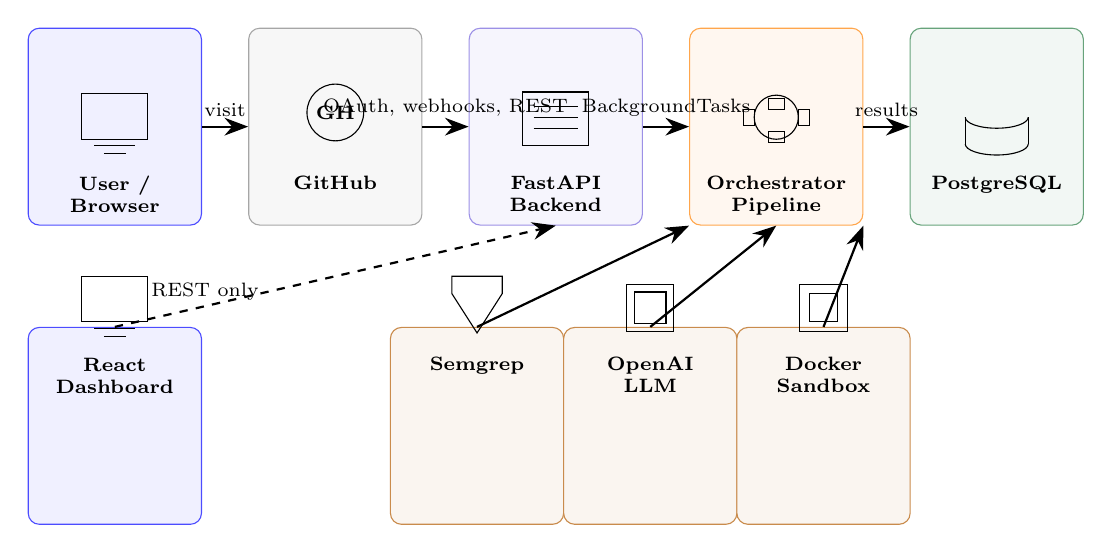
\begin{tikzpicture}[
  arrow/.style={-{Stealth[length=3mm]}, thick},
  block/.style={draw=#1!70, rounded corners, fill=#1!6,
                minimum width=2.2cm, minimum height=2.5cm},
  label/.style={font=\scriptsize\bfseries, anchor=north, align=center},
]
  % ---- Main horizontal chain ----
  \node[block=blue] (u) at (1.5,0) {};
    \draw (1.08,0.42) rectangle (1.92,-0.16);            % screen
    \draw (1.24,-0.24) -- (1.76,-0.24);                  % stand
    \draw (1.36,-0.34) -- (1.64,-0.34);                  % base
    \node[label] at (1.5,-0.5) {User /\\Browser};
  \node[block=gray] (gh) at (4.3,0) {};
    \draw (4.3,0.18) circle (0.36);
    \node at (4.3,0.18) {\scriptsize\bfseries GH};
    \node[label] at (4.3,-0.5) {GitHub};
  \node[block=quorumviolet] (fa) at (7.1,0) {};
    \draw (6.68,-0.24) rectangle (7.52,0.44);            % server rack
    \draw (6.82,-0.02) -- (7.38,-0.02);
    \draw (6.82,0.12) -- (7.38,0.12);
    \draw (6.82,0.26) -- (7.38,0.26);
    \node[label] at (7.1,-0.5) {FastAPI\\Backend};
  \node[block=orange] (or) at (9.9,0) {};
    \draw (9.9,0.12) circle (0.28);                      % gear
    \draw (9.48,0.02) rectangle (9.62,0.22);
    \draw (10.18,0.02) rectangle (10.32,0.22);
    \draw (9.8,-0.2) rectangle (10.0,-0.06);
    \draw (9.8,0.22) rectangle (10.0,0.36);
    \node[label] at (9.9,-0.5) {Orchestrator\\Pipeline};
  \node[block=quorumgreen!60!black] (db) at (12.7,0) {};
    \draw (12.3,-0.22) -- (12.3,0.12);
    \draw (13.1,-0.22) -- (13.1,0.12);
    \draw (12.3,0.12) arc (180:360:0.4 and 0.14);
    \draw (12.3,-0.22) arc (180:360:0.4 and 0.14);
    \node[label] at (12.7,-0.5) {PostgreSQL};

  % ---- Analysis services (below pipeline) ----
  \node[block=orange!70!black] (sg) at (6.1,-3.8) {};
    \draw (5.78,-1.9) -- (6.42,-1.9) -- (6.42,-2.12) -- (6.1,-2.62) -- (5.78,-2.12) -- cycle;
    \node[label] at (6.1,-2.8) {Semgrep};
  \node[block=orange!70!black] (llm) at (8.3,-3.8) {};
    \draw (8.0,-2.0) rectangle (8.6,-2.6);
    \draw (8.1,-2.1) rectangle (8.5,-2.5);
    \node[label] at (8.3,-2.8) {OpenAI\\LLM};
  \node[block=orange!70!black] (sb) at (10.5,-3.8) {};
    \draw (10.2,-2.0) rectangle (10.8,-2.6);
    \draw (10.32,-2.12) rectangle (10.68,-2.48);
    \node[label] at (10.5,-2.8) {Docker\\Sandbox};

  % ---- Dashboard (frontend) ----
  \node[block=blue] (ui) at (1.5,-3.8) {};
    \draw (1.08,-1.9) rectangle (1.92,-2.48);            % screen
    \draw (1.24,-2.56) -- (1.76,-2.56);
    \draw (1.36,-2.66) -- (1.64,-2.66);
    \node[label] at (1.5,-2.82) {React\\Dashboard};

  % ---- Arrows (main chain) ----
  \draw[arrow] (u.east) -- node[above, font=\scriptsize]{visit} (gh.west);
  \draw[arrow] (gh.east) -- node[above, font=\scriptsize]{OAuth, webhooks, REST} (fa.west);
  \draw[arrow] (fa.east) -- node[above, font=\scriptsize]{BackgroundTasks} (or.west);
  \draw[arrow] (or.east) -- node[above, font=\scriptsize]{results} (db.west);

  % ---- Arrows (services up to pipeline) ----
  \draw[arrow] (sg.north) -- (or.south west);
  \draw[arrow] (llm.north) -- (or.south);
  \draw[arrow] (sb.north) -- (or.south east);

  % ---- Dashboard REST arrow ----
  \draw[arrow, dashed] (ui.north) -- node[left, font=\scriptsize, pos=0.35]{REST only} (fa.south);
\end{tikzpicture}
\caption{Quorum architecture as an icon-block flow. The dashboard talks only to
the FastAPI backend; analysis services are driven by the orchestrator.}
\label{fig:architecture}
\end{figure}

\subsection{Component Description}

\begin{description}
  \item[GitHub] is the source of truth for pull requests. It delivers
  \texttt{pull\_request} webhook events, authorizes the user through OAuth,
  and provides installation-scoped repository access through the GitHub App.
  \item[FastAPI Backend] exposes the OAuth flow (\texttt{/auth/*}), the
  webhook endpoint (\texttt{POST /webhooks/github}, HMAC-verified), and the
  dashboard REST API (\texttt{/api/*}). It enforces user-level access
  isolation for every read and write.
  \item[Orchestrator / Review Pipeline] runs the registered analysis stages in
  a background task for each pull request. It creates an analysis run, marks
  it in progress, executes the stages, and records completion or failure.
  \item[Diff + AST] fetch and parse the pull request diff and the changed
  Python files to identify modified functions and classes.
  \item[Context] builds a bounded, prioritized prompt context from the changed
  files so that the LLM never receives an entire repository.
  \item[Semgrep] scans the changed files and produces structured JSON findings
  that form the security evidence.
  \item[Security Agent] (LLM) reasons over the Semgrep evidence and the code
  context, and produces structured findings that must be traceable to the
  evidence; it cannot invent findings.
  \item[Test Writer Agent] (LLM) generates \texttt{pytest} tests for the
  modified functions.
  \item[Docker Sandbox] executes the generated tests in a hardened container
  (no network, memory/process limits, hard timeout, guaranteed cleanup) and
  measures coverage before and after.
  \item[Synthesis] combines the security, test, and coverage results into the
  deterministic Merge Readiness Score, persists it with its breakdown, and
  builds the review comment that is posted back to GitHub.
  \item[PostgreSQL] persists all application data; it is accessed only by the
  backend.
  \item[React Web Dashboard] displays data through the FastAPI REST API and
  never accesses the database, Docker, Semgrep, the LLM, or GitHub directly.
\end{description}

\subsection{Why the Backend Is the System Boundary}

All privileged operations (GitHub tokens, database access, sandbox
execution, and LLM calls) require secrets or host access that must never be
exposed to the browser. By enforcing that the dashboard talks only to the
FastAPI REST API, the system keeps GitHub App tokens, the database, and the
analysis infrastructure out of the frontend and behind a single
authenticated boundary.

\section{User Flow}
\subsection{High-Level User Flow}

Figure~\ref{fig:userflow} shows the user flow as a swimlane diagram with three
lanes: the \textbf{User / Browser}, the \textbf{Quorum System}, and
\textbf{GitHub}. GitHub remains the source of truth: the user leaves Quorum
for GitHub OAuth and for the GitHub App installation flow, and GitHub delivers
pull request events back to Quorum through webhooks.

\begin{figure}[htbp]
\centering
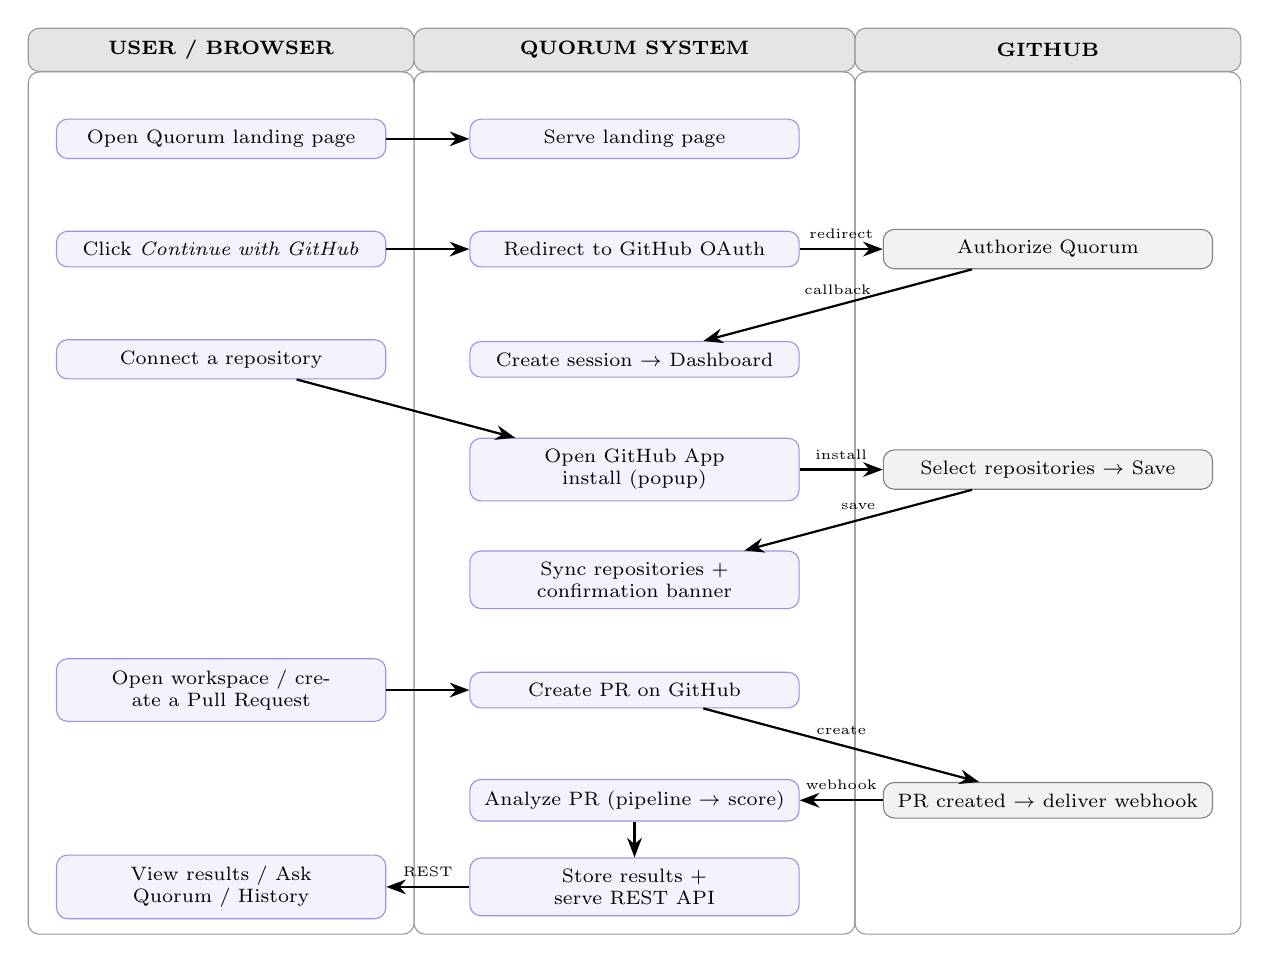
\begin{tikzpicture}[
  lane/.style={draw=black!40, rounded corners, fill=black!2},
  lanehdr/.style={draw=black!40, rounded corners, fill=black!10, font=\bfseries\scriptsize},
  sbox/.style={draw=quorumviolet!70, rounded corners, align=center,
               fill=quorumviolet!8, text width=3.9cm, inner sep=4pt, font=\scriptsize},
  gbox/.style={draw=gray, rounded corners, align=center,
               fill=gray!10, text width=3.9cm, inner sep=4pt, font=\scriptsize},
  arrow/.style={-{Stealth[length=2.5mm]}, thick},
]
  % ---- Lanes ----
  \draw[draw=black!40, rounded corners] (0,-0.55) rectangle (4.9,-11.5);
  \draw[draw=black!40, rounded corners] (4.9,-0.55) rectangle (10.5,-11.5);
  \draw[draw=black!40, rounded corners] (10.5,-0.55) rectangle (15.4,-11.5);
  \node[lanehdr, minimum width=4.9cm, minimum height=0.55cm] at (2.45,-0.27) {USER / BROWSER};
  \node[lanehdr, minimum width=5.6cm, minimum height=0.55cm] at (7.7,-0.27) {QUORUM SYSTEM};
  \node[lanehdr, minimum width=4.9cm, minimum height=0.55cm] at (12.95,-0.27) {GITHUB};

  % ---- Steps ----
  \node[sbox] (u1) at (2.45,-1.4) {Open Quorum landing page};
  \node[sbox] (q1) at (7.7,-1.4) {Serve landing page};

  \node[sbox] (u2) at (2.45,-2.8) {Click \emph{Continue with GitHub}};
  \node[sbox] (q2) at (7.7,-2.8) {Redirect to GitHub OAuth};
  \node[gbox] (g1) at (12.95,-2.8) {Authorize Quorum};

  \node[sbox] (q3) at (7.7,-4.2) {Create session $\rightarrow$ Dashboard};
  \node[sbox] (u3) at (2.45,-4.2) {Connect a repository};

  \node[sbox] (q4) at (7.7,-5.6) {Open GitHub App install (popup)};
  \node[gbox] (g2) at (12.95,-5.6) {Select repositories $\rightarrow$ Save};

  \node[sbox] (q5) at (7.7,-7.0) {Sync repositories + confirmation banner};

  \node[sbox] (u4) at (2.45,-8.4) {Open workspace / create a Pull Request};
  \node[sbox] (q6) at (7.7,-8.4) {Create PR on GitHub};

  \node[gbox] (g3) at (12.95,-9.8) {PR created $\rightarrow$ deliver webhook};
  \node[sbox] (q7) at (7.7,-9.8) {Analyze PR (pipeline $\rightarrow$ score)};

  \node[sbox] (q8) at (7.7,-10.9) {Store results + serve REST API};
  \node[sbox] (u5) at (2.45,-10.9) {View results / Ask Quorum / History};

  % ---- Arrows ----
  \draw[arrow] (u1) -- (q1);
  \draw[arrow] (u2) -- (q2);
  \draw[arrow] (q2) -- node[above, font=\tiny]{redirect} (g1);
  \draw[arrow] (g1) -- node[above, font=\tiny]{callback} (q3);
  \draw[arrow] (u3) -- (q4);
  \draw[arrow] (q4) -- node[above, font=\tiny]{install} (g2);
  \draw[arrow] (g2) -- node[above, font=\tiny]{save} (q5);
  \draw[arrow] (u4) -- (q6);
  \draw[arrow] (q6) -- node[above, font=\tiny]{create} (g3);
  \draw[arrow] (g3) -- node[above, font=\tiny]{webhook} (q7);
  \draw[arrow] (q7) -- (q8);
  \draw[arrow] (q8) -- node[above, font=\tiny]{REST} (u5);
\end{tikzpicture}
\caption{Swimlane user flow: the user alternates between Quorum and GitHub,
and GitHub returns control and events to Quorum.}
\label{fig:userflow}
\end{figure}

\subsection{Step-by-Step Explanation}

\begin{enumerate}[leftmargin=1.2em]
  \item \textbf{Landing page.} A public landing page introduces the product
        before authentication.
  \item \textbf{GitHub OAuth.} The user clicks \emph{Continue with GitHub},
        Quorum redirects to GitHub, and the user authorizes Quorum. GitHub
        redirects back and Quorum creates a server-side session.
  \item \textbf{Quorum dashboard.} The signed-in user lands on the dashboard.
  \item \textbf{Connect repository.} The user connects a repository. The
        GitHub App install page opens in a popup; when the user selects
        repositories and saves, GitHub redirects back, Quorum syncs the
        authorized repositories, and a confirmation banner appears.
  \item \textbf{Repository workspace / create PR.} The user opens a
        repository and creates a pull request from Quorum (Base/Compare
        branches, suggested title) or opens an existing one.
  \item \textbf{PR creation on GitHub.} Quorum creates the pull request on
        GitHub through the GitHub App API.
  \item \textbf{Webhook delivery.} GitHub delivers a \texttt{pull\_request}
        webhook to Quorum.
  \item \textbf{Analysis.} The orchestrator runs the review pipeline and
        stores the results (score, findings, tests, coverage).
  \item \textbf{Results.} The user views results, asks Ask Quorum questions,
        and returns to review history later.
\end{enumerate}

\section{Use Case Definition}
\subsection{Actors}

The main actors of the system are:

\begin{description}
  \item[Developer / User] --- the primary actor. A signed-in GitHub user who
        connects repositories, opens pull requests, and reviews analysis
        results.
  \item[GitHub] --- an external system that authenticates the user, hosts
        repositories and pull requests, and delivers webhook events.
  \item[GitHub App] --- the Quorum GitHub App installation that grants
        repository access; it participates in repository connection.
\end{description}

Internal components (the orchestrator, the analysis agents, the sandbox, and
PostgreSQL) are not treated as actors; they are implementation services that
run inside the Quorum system.

\subsection{Use Case Diagram}

Figure~\ref{fig:usecase} shows the use case model. All use cases are supported
by the current implementation.

\begin{figure}[htbp]
\centering
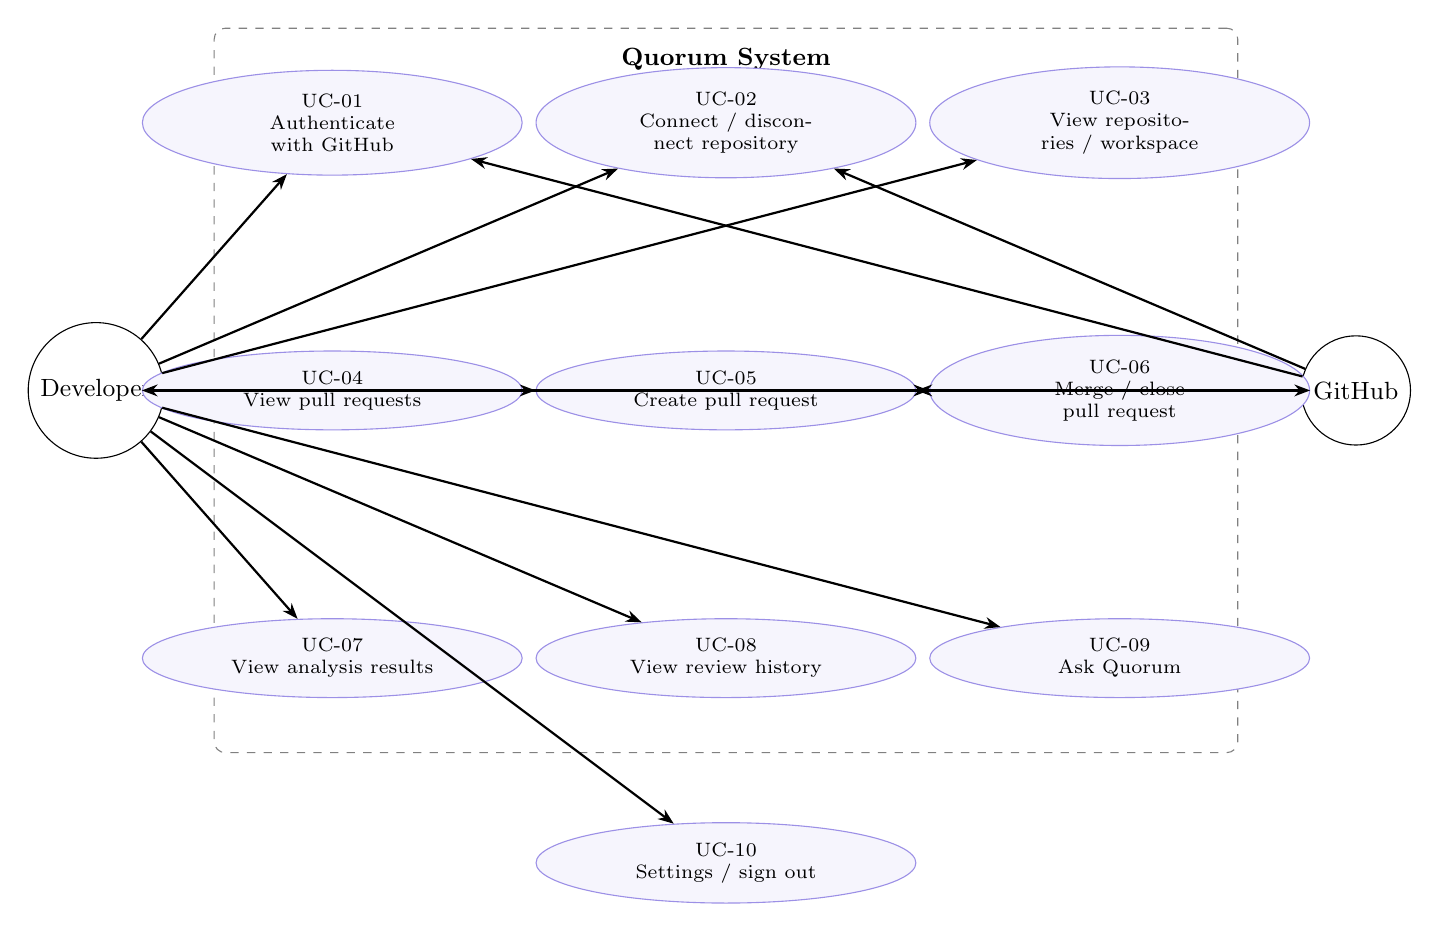
\begin{tikzpicture}[
  actor/.style={draw, circle, minimum size=0.9cm, font=\small},
  ellipse style/.style={draw=quorumviolet!70, ellipse, align=center,
              fill=quorumviolet!6, text width=3.2cm, inner sep=3pt, font=\scriptsize},
  arrow/.style={-{Stealth[length=2mm]}, thick},
]
  % Actors
  \node[actor] (dev) at (0,0) {Developer};
  \node[actor] (gh) at (16,0) {GitHub};

  % System boundary
  \node[draw=gray, rounded corners, dashed, minimum width=13cm,
        minimum height=9.2cm] (system) at (8,0) {};
  \node[font=\bfseries\small] at (8,4.2) {Quorum System};

  % Use cases (ellipses) inside the boundary
  \node[ellipse style] (uc1) at (3,3.4) {UC-01\\Authenticate with GitHub};
  \node[ellipse style] (uc2) at (8,3.4) {UC-02\\Connect / disconnect repository};
  \node[ellipse style] (uc3) at (13,3.4) {UC-03\\View repositories / workspace};
  \node[ellipse style] (uc4) at (3,0) {UC-04\\View pull requests};
  \node[ellipse style] (uc5) at (8,0) {UC-05\\Create pull request};
  \node[ellipse style] (uc6) at (13,0) {UC-06\\Merge / close pull request};
  \node[ellipse style] (uc7) at (3,-3.4) {UC-07\\View analysis results};
  \node[ellipse style] (uc8) at (8,-3.4) {UC-08\\View review history};
  \node[ellipse style] (uc9) at (13,-3.4) {UC-09\\Ask Quorum};
  \node[ellipse style] (uc10) at (8,-6) {UC-10\\Settings / sign out};

  % Developer to use cases
  \draw[arrow] (dev) -- (uc1);
  \draw[arrow] (dev) -- (uc2);
  \draw[arrow] (dev) -- (uc3);
  \draw[arrow] (dev) -- (uc4);
  \draw[arrow] (dev) -- (uc5);
  \draw[arrow] (dev) -- (uc6);
  \draw[arrow] (dev) -- (uc7);
  \draw[arrow] (dev) -- (uc8);
  \draw[arrow] (dev) -- (uc9);
  \draw[arrow] (dev) -- (uc10);

  % GitHub to relevant use cases
  \draw[arrow] (gh) -- (uc1);
  \draw[arrow] (gh) -- (uc2);
  \draw[arrow] (gh) -- (uc5);
  \draw[arrow] (gh) -- (uc6);
\end{tikzpicture}
\caption{Quorum use case diagram.}
\label{fig:usecase}
\end{figure}

\subsection{Use Case Definitions}

\subsubsection{UC-01 --- Authenticate with GitHub}
\begin{description}
  \item[Primary actor] Developer.
  \item[Supporting system] GitHub (OAuth).
  \item[Goal] The developer signs in and Quorum creates a session.
  \item[Preconditions] The developer has a GitHub account.
  \item[Trigger] The developer clicks \emph{Continue with GitHub}.
  \item[Main flow] The developer authorizes Quorum on GitHub; Quorum receives
        the OAuth callback, persists the user, and creates a session.
  \item[Postconditions] The dashboard shows the signed-in user.
\end{description}

\subsubsection{UC-02 --- Connect / Disconnect Repository}
\begin{description}
  \item[Primary actor] Developer.
  \item[Supporting system] GitHub App.
  \item[Goal] Grant (or revoke) Quorum access to a repository.
  \item[Preconditions] The developer is signed in.
  \item[Trigger] The developer clicks Connect or Disconnect on the
        repositories page or workspace.
  \item[Main flow] The GitHub App install/manage page opens in a popup; the
        developer selects repositories and saves; GitHub redirects back and
        Quorum syncs and shows a confirmation banner.
  \item[Postconditions] The repository is connected (or disconnected and
        remembered as such).
\end{description}

\subsubsection{UC-03 --- View Repositories / Workspace}
\begin{description}
  \item[Primary actor] Developer.
  \item[Goal] Browse connected repositories and open a repository workspace.
  \item[Main flow] The developer opens the Repositories page, sees connected
        and available repositories, and opens a repository to see its pull
        requests.
\end{description}

\subsubsection{UC-04 --- View Pull Requests}
\begin{description}
  \item[Primary actor] Developer.
  \item[Goal] See the pull requests of a repository with their analysis
        status.
  \item[Main flow] The developer opens a repository or the Pull Requests page
        and reviews the list.
\end{description}

\subsubsection{UC-05 --- Create Pull Request}
\begin{description}
  \item[Primary actor] Developer.
  \item[Supporting system] GitHub.
  \item[Goal] Create a real pull request on GitHub from Quorum.
  \item[Main flow] The developer selects Base and Compare branches (a title is
        suggested), adds a description, and submits; Quorum creates the pull
        request on GitHub and starts analysis.
  \item[Alternative] GitHub rejects the pull request; Quorum shows the error.
\end{description}

\subsubsection{UC-06 --- Merge / Close Pull Request}
\begin{description}
  \item[Primary actor] Developer.
  \item[Supporting system] GitHub.
  \item[Goal] Merge or close a pull request from Quorum.
  \item[Main flow] The developer chooses Merge (optionally with a message) or
        Close; Quorum performs the action on GitHub and the state is updated.
  \item[Alternative] The merge fails (for example conflict); Quorum shows the
        GitHub error.
\end{description}

\subsubsection{UC-07 --- View Analysis Results}
\begin{description}
  \item[Primary actor] Developer.
  \item[Goal] See the Merge Readiness Score, security findings, generated
        tests, and coverage for a pull request.
  \item[Main flow] The developer opens the PR review page; the results refresh
        automatically as analysis progresses.
\end{description}

\subsubsection{UC-08 --- View Review History}
\begin{description}
  \item[Primary actor] Developer.
  \item[Goal] Review previous analyses.
  \item[Main flow] The developer opens Review History and a previous review
        detail.
\end{description}

\subsubsection{UC-09 --- Ask Quorum}
\begin{description}
  \item[Primary actor] Developer.
  \item[Goal] Ask questions about a specific review.
  \item[Main flow] The developer asks a question on the review; the assistant
        answers using only that review's evidence.
\end{description}

\subsubsection{UC-10 --- Settings / Sign Out}
\begin{description}
  \item[Primary actor] Developer.
  \item[Goal] View account and connection status and sign out.
  \item[Main flow] The developer opens Settings, reviews GitHub account and
        connected repositories, and signs out.
\end{description}

\section{UI Screenshots}
This section references screenshots of the actual Quorum application. The
images are not included in the repository; they are placed manually into
\texttt{report/screenshots/} using the filenames listed in
\emph{SCREENSHOTS\_NEEDED.md}. If a file is missing, a placeholder box is
shown instead so the report still compiles.

\reportfigure{01-landing-page.png}{figure:screenshot-landing}{Landing Page}{The public landing page that introduces Quorum before authentication}

\reportfigure{02-github-login.png}{figure:screenshot-login}{GitHub Login}{The sign-in transition to GitHub OAuth}

\reportfigure{03-dashboard.png}{figure:screenshot-dashboard}{Dashboard}{The main dashboard with metrics, repositories, and pull requests}

\reportfigure{04-repositories.png}{figure:screenshot-repositories}{Repositories}{The repositories page with discovery and connection status}

\reportfigure{05-repository-workspace.png}{figure:screenshot-workspace}{Repository Workspace}{A connected repository's workspace showing its pull requests}

\reportfigure{06-pull-requests.png}{figure:screenshot-pull-requests}{Pull Requests}{The pull request list with analysis status}

\reportfigure{07-pr-review-details.png}{figure:screenshot-pr-review}{Pull Request Review Details}{The review page with score, findings, tests, and coverage}

\reportfigure{08-security-findings.png}{figure:screenshot-findings}{Security Findings}{Security findings with severity, location, and evidence}

\reportfigure{09-test-results.png}{figure:screenshot-tests}{Generated Test Results}{Generated tests and their pass/fail outcomes}

\reportfigure{10-coverage.png}{figure:screenshot-coverage}{Coverage}{Coverage before/after and delta for a review}

\reportfigure{11-review-history.png}{figure:screenshot-history}{Review History}{The list of previous analyses}

\reportfigure{12-ask-quorum.png}{figure:screenshot-ask}{Ask Quorum}{The evidence-grounded question-answering assistant}

\reportfigure{13-settings.png}{figure:screenshot-settings}{Settings}{GitHub account, connected repositories, and sign out}

\end{document}